%\documentclass[jou]{apa6}
\documentclass[11pt]{article}
\usepackage{ucs}
\usepackage[utf8x]{inputenc}
\usepackage{changepage}
\usepackage{graphicx}
\usepackage{amsmath}
\usepackage{gensymb}
\usepackage{amssymb}
\usepackage{enumerate}
\usepackage{tabularx}
\usepackage{lipsum}
\usepackage{hyperref}
\usepackage{fancyvrb}

\oddsidemargin 0.0in
\evensidemargin 0.0in
\textwidth 6.27in
\headheight 1.0in
\topmargin -0.1in
\headheight 0.0in
\headsep 0.0in
\textheight 9.0in

\usepackage{xcolor}

\setlength\parindent{0pt}

\newenvironment{myenv}{\begin{adjustwidth}{0.4in}{0.4in}}{\end{adjustwidth}}
\renewcommand{\abstractname}{Anotācija}
\renewcommand\refname{Atsauces}



\newcounter{alphnum}
\newenvironment{alphlist}{\begin{list}{(\Alph{alphnum})}{\usecounter{alphnum}\setlength{\leftmargin}{2.5em}} \rm}{\end{list}}


%16.3-6

\makeatletter
\let\saved@bibitem\@bibitem
\makeatother

\usepackage{bibentry}



\begin{document}
\thispagestyle{empty}


\begin{center}
{\Large C++ Exercise 6: Shapes and Transformations}
\end{center}

%\begin{abstract}
%This exercise shows how to implement a circularly linked list 
%of integers. 
%% https://softwareengineering.stackexchange.com/questions/149555/difference-between-immutable-and-const
%% Our rational numbers are "immutable"
%\end{abstract}


{\bf Deadline:} Monday, October 26, 2020 by 23:59:59 EET Timezone.\\ 
{\bf How to submit:} Check your code into your GitHub repository, 
the default {\tt master} branch, 
tag it as {\tt ex06submit} (all lowercase, no dashes).\\
{\bf Grading:} This exercise is worth 3\textperthousand (or $3\%$) of the total grade.\\
{\bf Objectives:} Develop a software that receives a list of commands on separate lines that define shapes 
(either regular $n$-gons or circles), apply transformations to those shapes, 
copy and group the shapes and finally paint them as SVG.


\vspace{20pt}
{\bf \large Two Stages}

It is suggested that you do this lab in two stages. 
Each stage will have unit tests, so that you can check yourself. 
You are welcome to use other implementations as well; 
so you can also ignore this suggestion, if you know a better way.
 
\begin{enumerate}
\item During the first stage you check if you can create some basic shape 
(for example a polygon), apply one or more transformations to that 
basic shape and draw the shape as an SVG. During this stage you 
can try out, if you can create transformation matrices of all kinds and 
understand the SVG output.
\item During the second stage you can create groups of shapes and see, if 
you can transform and draw entire groups (and also nested groups of groups) 
using the {\em Composite} design pattern and virtual functions
{\tt transform()} and {\tt draw()}.
You will have abstract {\tt Shape} class, and also its child class {\tt Group}
that can contain other shapes (circles, polygons and other groups).  
\end{enumerate}



\vspace{20pt}
{\bf \large Description}

Assume that we need to draw groups of simple shapes such as circles, 
rectangles, triangles (and some other polygons such as stars).
We start from just two kinds of ``basic shapes'' 
(circles and regular polygons) \textendash{} they can be created 
in any color by specifying their RGB color coordinates. 

We can transform 
these shapes by multiplying their vertices $(x,y,1)$
by $3 \times 3$ transformation matrices 
(to support translations, rotations, scaling and sharing). 
We can also group shapes together: Each group can consist of basic shapes
(after they have received one or or more transformations), 
and also a group can obtain other groups. 

This editing process is similar to what you would do in a  
graphics editor (you can resize, drag or rotate shapes and combine them 
in groups on multiple levels). After you have grouped together the shapes 
you want, they are 


Then they are output to a vector graphics format (SVG). 
We want to do all coordinate transformations (such as translating 
the coordinates) inside our C++ program using matrix multiplication. 
(I.e. we avoid any coordinate transformation operations in the SVG itself; 
it only displays closed paths from points that are already transformed.)


\vspace{20pt}
{\bf \large Transformations}

There are only two types of basic shapes that can be created: it is either 
a unit circle (circle with center in $(0,0)$ and radius $1$) or 
a regular $n$-gon (where $n \geq 3$; 
one of the $n$-gon's vertices is always $(1,0)$ - the point on the $X$ axis
and its center is point $(0,0)$). See Figure~\ref{fig:ex06-basic-shapes}


\begin{figure}[!htb]
\center{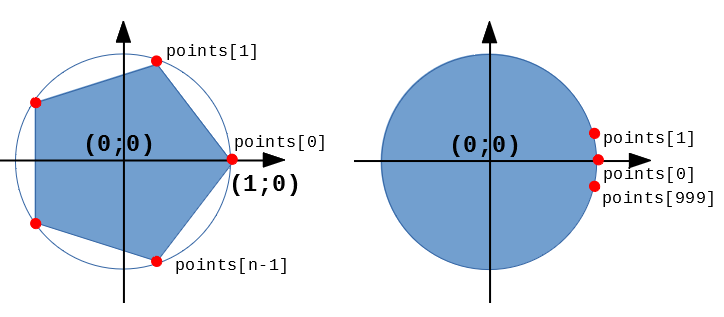
\includegraphics[width=3in]{ex06-basic-shapes.png}}
\caption{\label{fig:ex06-basic-shapes} Polygon (here $n=5$) and Circle before any transformations.}
\end{figure}


All the other shapes are obtained from these two basic shapes by applying 
some linear coordinate transformations. 
See \url{https://bit.ly/30Yq3xN} - Affine transformations for 2D images. 
There are just 4 transformations: 

\begin{itemize}
\item Translation denoted by {\tt TRA dx dx}: it shifts all points in a shape by a vector $(dx,dy)$
\item Rotation denoted by {\tt ROT alpha}: it rotates all points in a shape by angle {\tt alpha} degrees
around the center $(0,0)$.
\item Scaling denoted by {\tt SCA cx cy}: it multiplies coordinates of all points in a shape
by {\tt cx} and {\tt cy} respectively. The numbers {\tt cx,cy} can be negative; we can 
also get mirror images of the original figure.
\item Shearing denoted by {\tt SHE cx cy}: it maps every point $(x,y)$ to a point
$(x + cx \cdot y, y + cy \cdot x)$. 
\end{itemize}

\vspace{20pt}
{\bf \large Input and Output}

Input files contain the following commands. 

\begin{itemize}
\item Commands {\tt CIRCLE \#ABCDEF} or {\tt POLYGON \#ABCDEF n} push a new unit circle or a unit $n$-gon 
to the top of the stack; its color is defined by the RGB color coordinates ({\tt \#000000} is black, 
{\tt \#FF0000} is red and so on.). 
\item Commands {\tt TRANSF TRA dx dy}, {\tt TRANSF SCA cx cy}, etc. apply one of the 
linear transformations to the shape that is at the top of the stack. 
\item Command {\tt COPY} takes the element at the top of the stack, makes a deep copy of it and
pushes it to the top of the stack. 
\item Command {\tt GROUP N} pops the top $N$ elements off the stack, makes a group of these 
elements and pushes this as a group back to the stack. 
\item Command {\tt SHOW width height} pops the top element off the stack and outputs an SVG image with 
size {\tt width} by {\tt height} pixels.
\end{itemize}


\vspace{20pt}
{\bf \large  Limitations}

You can assume the following:

\begin{enumerate}
\item The total number of shapes (basic shapes or groups) ever pushed to the stack does not exceed $1000$. 
\item No polygon will have more than $1000$ sides.
\item Under transformations defined above, circles can be 
implemened as regular polygons with many vertices
(for example, $1000$ vertices). The test data will not apply extreme 
streching to those circles that would expose this workaround.
\item The width and the height is between $100$ to $1000$ pixels; borders of width $1$ are visible. 
\item Grouping in the input files does not cause exceptions ({\tt pop()} on an empty stack). 
\end{enumerate}


\vspace{20pt}
{\bf \large Implementation Details}

\begin{enumerate}
\item Implement whatever CPP and H files you need
(most likely you will need {\tt ShapesMain.cpp} as your main method, 
{\tt Circle.cpp}, {\tt Circle.h}, {\tt Polygon.cpp}, {\tt Polygon.h}, 
{\tt Group.cpp}, {\tt Group.h} (group of shapes), 
{\tt Shape.cpp} (abstract shape parent for circles, polygons and groups), 
{\tt Matrix.h} (to implement matrix multiplication for doubles; you can 
also store point coordinates as matrices, if you want), 
{\tt Stack.cpp} (some stack implementation; you can use a large array; 
you can assume that the stack size never exceeds $1000$ entries).
\item Inside the group you can store the children as an 
array of {\tt Shape*} (pointers to shapes, including other groups).
\item Implement the composite pattern to apply geometric transformations
for shapes, including nested shape groups. 
\end{enumerate}

\vspace{20pt}
{\bf \large Sample Input and Output}\\


\vspace{10pt}
\begin{tabular}{@{}ll@{}}
\begin{minipage}[t]{0.49\columnwidth}
Sample input {\bf test01in.txt}:
\begin{verbatim}
POLYGON #FFFFF 4
TRANSF ROT 45
TRANSF SCA 1.4142135 1.4143135
TRANSF SCA 150 100
TRANSF TRA 150 100
CIRCLE #BC002D
TRANSF SCA 60 60
TRANSF TRA 150 100
GROUP 2
SHOW 300 200
\end{verbatim}
\end{minipage} 
&
\begin{minipage}[t]{0.49\columnwidth}
Expected output {\bf test01expected.svg}:\\
\center{
\includegraphics[width=2in]{japan.png}}
\end{minipage} 
\end{tabular}


\vspace{10pt}
\begin{tabular}{@{}ll@{}}
\begin{minipage}[t]{0.49\columnwidth}
Sample input {\bf test02in.txt}:
\begin{verbatim}
POLYGON #FFFFFF 4
TRANSF ROT 45
TRANSF SCA 1.4142135 1.4143135
TRANSF TRA 0 -1
POLYGON #D7141A 4
TRANSF ROT 45
TRANSF SCA 1.4142135 1.4143135
TRANSF TRA 0 1
GROUP 2
TRANSF SCA 150 50
TRANSF TRA 150 100
POLYGON #11457E 3
TRANSF TRA 0.5 0
TRANSF SCA 115.4701 115.4701
TRANSF TRA 0 100
GROUP 2
SHOW 300 200
\end{verbatim}
\end{minipage} 
&
\begin{minipage}[t]{0.49\columnwidth}
Expected output {\bf test02expected.svg}:\\
\center{
\includegraphics[width=2in]{czech.png}}
\end{minipage} 
\end{tabular}





\vspace{20pt}
{\bf \large  Standard Output as an SVG File}

You need to know just two SVG elements in order to complete this task. 
SVG is a rich vector-graphics language that has its own mechanisms to do 
coordinate transformations, but we are not using them here, since all 
the point coordinates will be computed in your C++ code. 

{\bf What is the painting order in SVG:}\\
This exercise does not use special SVG parameters to affect the painting 
order (such as the CSS property {\tt z-index}). 
By default the shapes ({\tt path} elements) 
in SVG are painted on top of each other in the order in which they 
appear in the document you output.
For the Japanese flag you would first paint the white rectangle and then 
the red circle. 

If you use stacks in {\bf two} places (Firstly, to accumulate the shapes 
received in the input, Secondly, to store child elements in your groups), 
the shape order is reversed twice. So they will be painted 
in the same order as you specify them in the input file. 

%\begin{figure}[!htb]
%\center{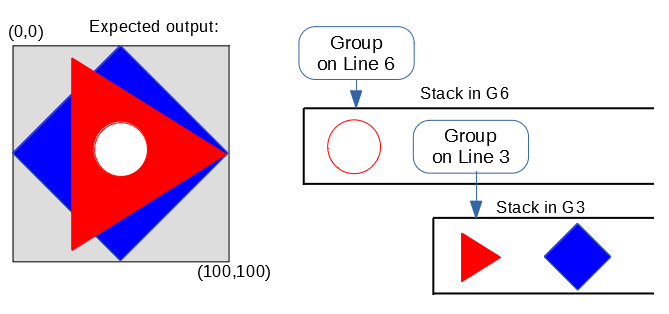
\includegraphics[width=3in]{ex06-overlapping-shapes.png}}
%\caption{\label{fig:ex06-overlapping-shapes} Three overlapping shapes.}
%\end{figure}


In this example, the input file contains shapes in the order we want them stacked
(first the blue square, then the red triangle, finally the white circle). 





\begin{tabular}{@{}ll@{}}
\begin{minipage}[t]{0.29\columnwidth}

\begin{Verbatim}[frame=single,numbers=left]
POLYGON #0000FF 4
POLYGON #FF0000 3
GROUP 2
CIRCLE #FFFFFF
TRANSF SCA 0.25 0.25
GROUP 2
TRANSF SCA 50 50
TRANSF TRA 50 50
SHOW 100 100
\end{Verbatim}

\end{minipage} 
&
\begin{minipage}[t]{0.57\columnwidth}
\center{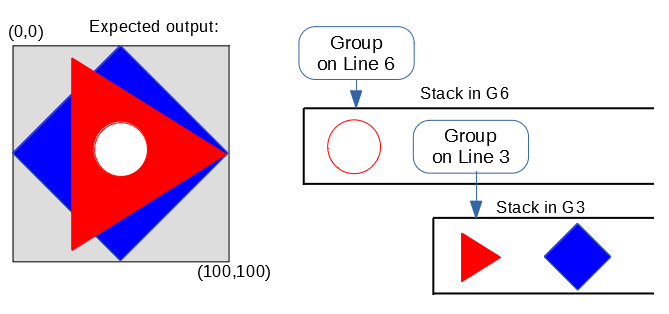
\includegraphics[width=4in]{ex06-overlapping-shapes.png}}
\end{minipage} 
\end{tabular}






In the Group3 (created on input Line 3) 
red triangle is pushed into the Group3 first (as in the Line 3 it popped out
the input stack), followed by the blue square. 
In the Group 6 (created on input Line 6), the white circle is pushed 
into its stack first; followed by Group3 that was created before. 
As you call {\tt draw()} function, they are drawn in the correct order again: 
first the blue square, then the red triangle, finally the white circle.


\vspace{20pt}
{\bf \large Testing your Code}\\
Unlike many previous exercises it is not easy to check real-valued matrix multiplication 
results using Linux {\tt diff} utility; the rounding errors are not always predictable. 
It is expected that different students can get slightly different outputs. 
For this reason the testing of this program 
is best done by inspecting the generated images. 

One or more SVG outputs can be embedded in an HTML file:

\begin{tabular}{@{}ll@{}}
\begin{minipage}[t]{0.49\columnwidth}

\begin{Verbatim}[frame=single,numbers=left]
<html>
<head>
<title>Embedded SVG</title>
</head>
<body>
<img src="image.svg"/>
</body>
</html>
\end{Verbatim}

\end{minipage} 
&
\begin{minipage}[t]{0.45\columnwidth}
\mbox{}\\[-20pt]
\center{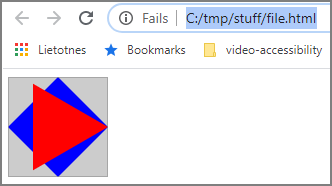
\includegraphics[width=2.5in]{svg-embedded.png}}
\end{minipage} 
\end{tabular}




The file {\tt image.svg} is shown below. 
The ``interesting'' part of the SVG is on Lines 4 and 5 only - it 
draws two polygons. (The first two lines define a light-gray canvas 
of size $100 \times 100$. 
The last {\tt <rect>} element draws a darker-gray rectangle 
around the image.)

All the polygons and circles need just one SVG element {\tt path}. 
It has attribute {\tt d} that has a long list of
commands followed by coordinates (and also ability to specify the fill shape). 
For example, {\tt M 100 50} moves the pencil to the specified coordinates $(100,50)$; 
command {\tt L 50 0} draws a line to a new point $(50,0)$ and so on. 
Please note that the $y$ axis in SVG goes downwards. 

\renewcommand{\FancyVerbFormatLine}[1]{%
  \ifnum\value{FancyVerbLine}=4
    \textcolor{blue}{#1}% Format specific line
  \else
	\ifnum\value{FancyVerbLine}=5
      \textcolor{red}{#1}% Format specific line
    \else	
    #1% Else, do nothing different
	\fi
  \fi
}

\begin{Verbatim}[frame=single,numbers=left]
<?xml version="1.0" encoding="UTF-8"?>
<svg xmlns="http://www.w3.org/2000/svg" width="100" height="100">
<path d="M 0 0 L 100 0 L 100 100 L 0 100" fill="#cccccc"/>
<path d="M 100 50 L 50 0 L 0 50 L 50 100" fill="#0000ff"/>
<path d="M 100 50 L 25 93.3 L 25 6.7" fill="#ff0000"/>
<rect x="0" y="0" width="100" height="100" 
stroke="#999999" fill="none" stroke-width="1"/>
</svg>
\end{Verbatim}



{\em Note.} You can draw the circles using same {\tt path} command as well 
(treating them as polygons with $1000$ vertices). 
Therefore you would need just the {\tt path} element in SVG (and its commands 
"M" - move to, "L" - line to).
(There are many other SVG elements to create advanced visualizations, but they are
outside the scope. In EX06 we only care about the data structures 
to compute the point coordinates inside the C++ program itself; SVG is used just 
to show the closed paths.) 

\vspace{20pt}
{\bf \large Suggested Object Model}

Please note that there are no restrictions on the implementation as long as you
can read the input files and output the transformed shapes as SVG (so you can safely ignore
this section). 

In the diagram (see Figure~\ref{fig:ex06-uml-diagram}) we try to implement a few 
object-orientation patterns and some other tricks. Here is the list:

\begin{enumerate}
\item 
The shapes are built using \textcolor{blue}{\em Composite Pattern}:
{\tt Shape} is an abstract class that materializes 
as {\tt Group}, {\tt Circle}, {\tt Polygon}; and {\tt Group} itself may contain other shapes, 
including other groups. Calling methods {\tt draw()} or {\tt transform()} on a {\tt Group} objects, 
they recursively propagate down the tree: In order to transform a group of shapes (e.g.\ to rotate 
some group), we call the same transform on every member of that group.
\item 
The methods to manipulate shapes are implemented using \textcolor{blue}{\em Abstract class}
and \textcolor{blue}{\em Pure virtual method} language constructs. The top-level class {\tt Shape} 
does not know how to draw itself or how to transform itself (consequently, one 
cannot create objects of this type). Fortunately, the 
derived classes ({\tt Circle}, {\tt Polygon} or {\tt Group}) consist of concrete points
and other shapes, so they can draw/transform themselves.
\item 
Handling objects of various types by the same code is called \textcolor{blue}{\em Polymorphism}. 
For example, iterating over shapes of different kinds in {\tt ShapeStack} is a particular case of polymorphism.
Virtual methods ensure that we can call methods like {\tt draw()} and {\tt transform()} on 
these shapes (and each shape will know, how to apply the method correctly).
\item 
The transformation matrices are created using \textcolor{blue}{\em Factory Pattern}: 
we want to allow creating matrices in just one class: {\tt Transformation}. 
Creation of $3 \times 3$  matrices for affine transformations
do not depend on any ``state of object'', so they can use 
\textcolor{blue}{\em Static Methods}. 
For example, if you want to rotate vector $\mathbf{v}=(x,y)=(3,5)$ by $72^{\circ}$
and get another vector $\mathbf{w}=(x',y')$, you can write it like this:
\begin{verbatim}
Matrix<double> mm = Transformation::getROT(72); // 3x3 matrix
Matrix<double> vv(3,1); // column vector has 3 rows, 1 column
vv.a[0][0] = 3; vv.a[1][0] = 5; vv.a[2][0] = 1; 
Matrix<double> ww = mm*vv;
\end{verbatim}
This code is cleaner and shorter (compared to calling matrix constructor directly and filling 
all the $3 \times 3 =9$ entries manually). 
\item 
In the UML diagram the collection used is \textcolor{blue}{\em Iterable Stack} \textendash{}
see the class diagram for {\tt ShapeStack}. In addition to all the stack-specific methods
(push, pop, etc.) it should also allow to iterate. For example, if we want to apply 
some affine transformation to all members of some group. 
Our input handling (and also correct drawing order) depends on the stack behavior. 
On the other hand ``vanilla'' stack has very limited set of methods: The stack from 
your textbook does not support iteration (visiting all elements) easily: You can 
only look at the top element (and to look deeper you need to pop off the top elements).\\
To work around this you can either manipulate two stacks (pop off one of them, push into another one; 
then do same thing backwards \textendash{} to restore the correct order). 
But you can also provide an additional ``iterator cursor'' variable in the stack that can 
move around and visit all elements in your stack (without destroying them).
Such iterable stacks are sometimes discussed in data structures courses:
\url{https://introcs.cs.princeton.edu/java/43stack/}. 
\item Our UML diagram uses some new notation (class inheritance shown as 
a white triangle; aggregation 
shown as a white diamond and association shown as simple line). Their differences
are explained here - \url{https://bit.ly/31vjbbJ}.
\end{enumerate}


As usual, the private members (grayed out in the diagram) is something 
that developers of this diagram can do in whichever way they want;
due to encapsulation not even unit tests can test private members. 
(And you are responsible for reading the STDIN and printing SVG to STDOUT; 
so let's stress it once more that you should feel free to change this suggested 
class design any way you want.)


 

\begin{figure}[!htb]
\center{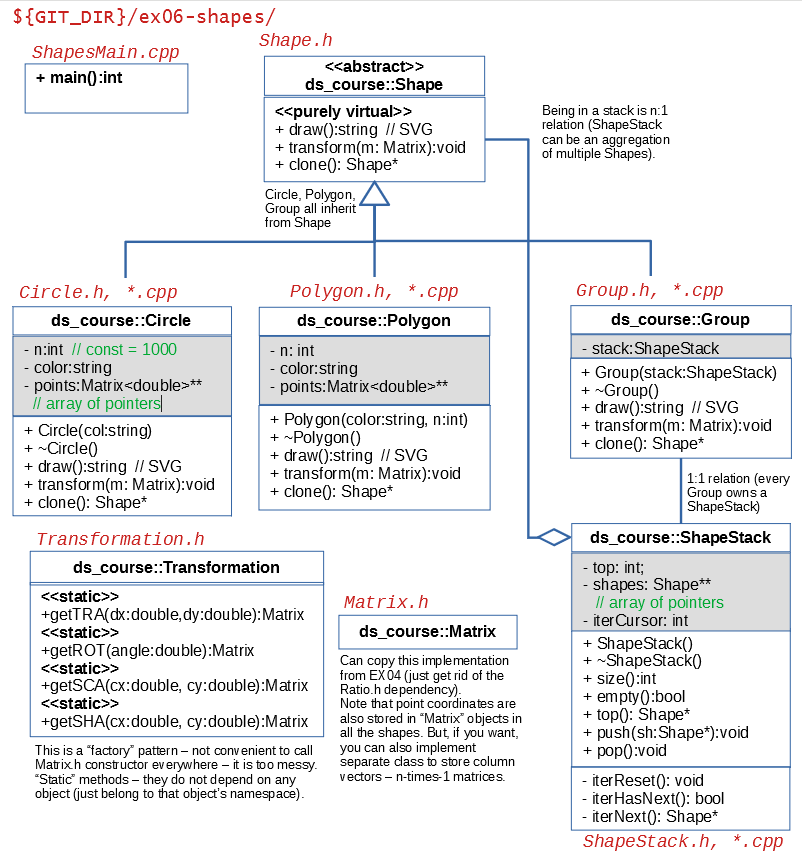
\includegraphics[width=5in]{ex06-uml-diagram.png}}
\caption{\label{fig:ex06-uml-diagram} Suggested UML Diagram}
\end{figure}


\vspace{20pt}
{\bf \large Some Pseudocode}

Finally, once the object model (with its classes and their interfaces 
and iterable stack interface with its Abstract Data Type (ADT)) is ready, 
we can try to show, how this can be put together to parse the input files 
and to do the requested actions. 


\[
\begin{array}{rl}
 & \text{\textsc{Main()}}:\\
1 & s \leftarrow empty\;\mathtt{ShapeStack}\\
2 & \text{\textbf{while\ }} (getline( cin, Line)):\;\;\text{\em (Can read one more line)}\\
3 & \hspace{.5cm} cmd \leftarrow \text{token from $Line$}\;\;\text{\em (Read command-name)}\\
4 & \hspace{.5cm} \text{\textbf{if\ } cmd == {\tt "CIRCLE"}}\\
5 & \hspace{1.0cm} color \leftarrow \text{token from $Line$}\\
6 & \hspace{1.0cm} s.push(new\;\;Circle(color))\\
7 & \hspace{.5cm} \text{\textbf{if\ } cmd == {\tt "POLYGON"}}\\
8 & \hspace{1.0cm} (color,n) \leftarrow \text{$2$ tokens from $Line$}\\
9 & \hspace{1.0cm} s.push(new\;\;Polygon(color,n))\\
10 & \hspace{.5cm} \text{\textbf{if\ } cmd == {\tt "TRANSF"}}\\
11 & \hspace{1.0cm} (type,cx,cy) \leftarrow \text{$2$ or $3$ tokens from $Line$}\;\;\text{\em (rotation needs just angle)}\\
12 & \hspace{1.0cm} matrix \leftarrow Transformation::getROT(angle)\;\;\text{\em (or any other transformation matrix)}\\
13 & \hspace{1.0cm} s.top().transform(matrix)\;\;\text{\em (apply to the stack's top element only)}\\
14 & \hspace{0.5cm} \text{\textbf{if\ } cmd == {\tt "COPY"}}\\
15 & \hspace{1.0cm} newShape \leftarrow s.top().clone\\
16 & \hspace{1.0cm} s.push(newShape)\\
17 & \hspace{0.5cm} \text{\textbf{if\ } cmd == {\tt "GROUP"}}\\
18 & \hspace{1.0cm} N \leftarrow \text{token from $Line$}\\
19 & \hspace{1.0cm} gStack \leftarrow empty\;\mathtt{ShapeStack}\\
20 & \hspace{1.0cm} \text{\textbf{repeat $N$ times}}\\
21 & \hspace{1.5cm} shp \leftarrow s.top()\\
22 & \hspace{1.5cm} s.pop()\\
23 & \hspace{1.5cm} gStack.push(shp)\\
24 & \hspace{1.0cm} s.push(new\;\;Group(gStack))\\
25 & \hspace{0.5cm} \text{\textbf{if\ } cmd == {\tt "SHOW"}}\\
26 & \hspace{1.0cm} \text{\textbf{output\ }} s.top().draw()\;\;\;\text{\em (surround with a few more SVG lines)}\\
27 & \hspace{1.0cm} \text{\textbf{return\ }} 0\\
\end{array}
\]



\vspace{10pt}
A sample, how ``iterable stack'' can be used. Transform 
a group by transforming each element:

\[
\begin{array}{rl}
 & \text{\textsc{Group::transform}}(matrix):\\
1 & s \leftarrow \text{group's instance of {\tt ShapeStack}} \hspace{8.7cm} \mbox{}\\
2 & s.iterReset()\\
3 & \text{\textbf{while\ }} s.iterHasNext()\\
4 & \hspace{0.5cm} s.iterNext().transform(matrix)
\end{array}
\]


\end{document}







